\documentclass[dvipdfmx]{jarticle}

\usepackage[letterpaper,top=2cm,bottom=2cm,left=3cm,right=3cm,marginparwidth=1.75cm]{geometry}
\usepackage{itembkbx}
\usepackage{boites,boites_exemples}
\usepackage{lipsum}
% Useful packages
\usepackage{amsmath}
\usepackage{graphicx}
\usepackage[colorlinks=true, allcolors=blue]{hyperref}
\usepackage{ascmac}
\usepackage[many]{tcolorbox}
\tcbuselibrary{breakable, skins, theorems}
\usepackage{color}
\usepackage{xcolor}
\usepackage{listings}
\lstset{%
  language={Python},
  basicstyle={\small},%
  identifierstyle={\small},%
  commentstyle={\small\itshape\color[rgb]{0,0.5,0}},%
  keywordstyle={\small\bfseries\color[rgb]{0,0,1}},%
  ndkeywordstyle={\small},%
  stringstyle={\small\ttfamily\color[rgb]{1,0,1}},
  frame={tb},
  breaklines=true,
  columns=[l]{fullflexible},%
  numbers=left,%
  xrightmargin=0zw,%
  xleftmargin=3zw,%
  numberstyle={\scriptsize},%
  stepnumber=1,
  numbersep=1zw,%
  lineskip=-0.5ex%
}
\usepackage{tikz}
\usetikzlibrary{shapes.geometric}
\usetikzlibrary {shapes.misc}
\usetikzlibrary{positioning}
\title{最大公約数の計算}
\author{}
\date{}
\begin{document}
\maketitle
最大公約数は二つの自然数の公約数のうち最大の自然数です。
このコードでは与えられた2つの自然数の最大公約数の計算ア
ルゴリズムをいくつか実装しました。このコードでは継承と汎化の方法を使って
最大公約数を計算する基底クラスgcd\_baseを抽象クラスとして定義し、
gcd\_baseクラスを継承する形で実際のアルゴリズムを行うクラスを実装しました。
\begin{lstlisting}[caption=gcd\_base,label=base]
class gcd_base(metaclass = ABCMeta):
    def __init__(self)->None:
        pass
    @abstractmethod
    def get(self)->int:
        pass

    def check_parameter(self,a:int,b:int)->bool:
        if a<=0 or b<=0:
            print("a and b must be positive!!")
            return False
        return True
 \end{lstlisting}
この規定クラスではget抽象メソッドを定義しています。このメソッドは汎化した先で
それぞれの最大公約数を計算するアルゴリズムを実装します。基底クラスではアルゴリズムを
指定していないのでgetメソッドを定義することができないので抽象メソッドとしています。
またcheck\_parameterというメソッドも定義しました。こちらは二つの数字が正の整数かどうか
を判断するメソッドです。このメソッドは汎化先のどのクラスでも共通なので基底クラスの方に
定義しました。

それではこのgcd\_baseクラスを継承したクラスを見ていきます。
\begin{itemize}
\item simple\_gcd
最初のクラスはsimple\_gcdというクラスで実装しました。
\end{itemize}
\begin{lstlisting}[caption=gcd\_simple,label=simple]
class simple_gcd(gcd_base):
    def __init__(self)->None:
        super().__init__()

    def get(self,a:int,b:int)->int:
        if not super().check_parameter(a,b):
            return 0
        if a < b:
            a,b = b,a
        x=b
        while True:
            if a%x == 0 and b%x==0:
                return x
            x-=1
 \end{lstlisting}
 こちらのクラスでは与えられた自然数a,bに対する最大公約数はa,bより小さいことがわかっているので、
 min(a,b)から順番にマイナス1していき最大公約数を計算しています。
 \begin{itemize}
\item gcd\_eucidean
\end{itemize}
二つ目の方法はgcd\_eucideanというクラスで実装しています。
\begin{lstlisting}[caption=gcd\_eucidean,label=euclidean]
 class euclidean_algo(gcd_base):
    def __init__(self)->None:
        super().__init__()

    def get(self,a:int,b:int)->int:
        if not super().check_parameter(a,b):
            return 0
        if a < b:
            a,b = b,a
        while True:
            r = a%b
            if r==0:
                return b
            a,b = b,r
 \end{lstlisting} 
 こちらの方法ではユークリッド互除法を用いて計算しています。
 
 最後にkの二つのアルゴリズムのTATを計測しました。
 \begin{figure}[h]
 \begin{center}
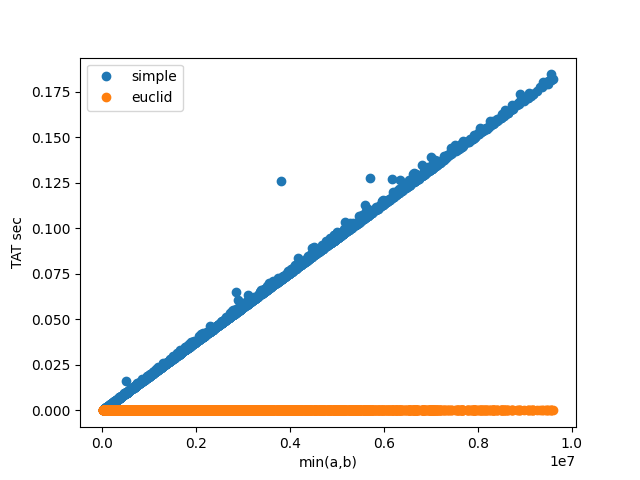
\includegraphics[width=100mm]{time_measure.png}
\end{center}
\end{figure}

\begin{thebibliography}{9}
\item 辻真吾、下平英寿、「Pythonで学ぶアルゴリズムとデータ構造」
\end{thebibliography}

\end{document}
